\chapter{Clystyru $k$-cymedr}\label{cha:literature}
\section{Cefndir}
Mae clystyru $k$-cymedr yn ffordd o ddysgu heb oruchwyliaeth, mae'n cymryd data heb ei labelu ac yn eu sortio i mewn i $k$ wahanol glwstwr yn yr obaith i ddarganfod rhyw strwythur doedden ddim yn gwybod yn gynharach.

\begin{figure}
\begin{center}
\begin{minipage}{.4\linewidth}
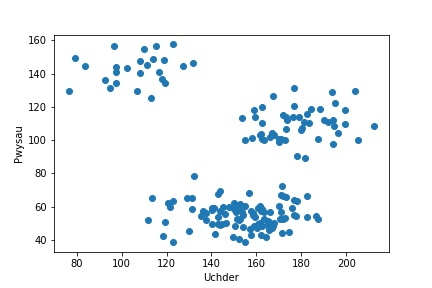
\includegraphics[width=1\linewidth]{../img/Scatterpython.jpeg}
\end{minipage}%
\begin{minipage}{1cm}
$\Rightarrow$
\end{minipage}%
\begin{minipage}{.4\linewidth}
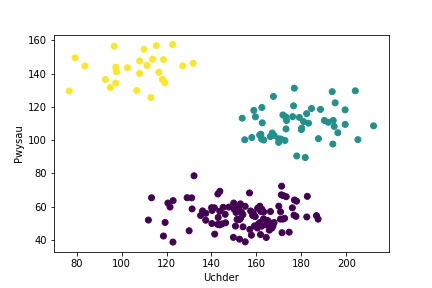
\includegraphics[width=1\linewidth]{../img/3clystwrpython.jpeg}
\end{minipage}%
\label{fig:Cefndir_Clysteru_k_modd}
\caption{Cyn ac ar \^{o}l clystyru $k$-cymedr.}
\end{center}
\end{figure}

I roi enghraifft gwelwch Ddarlun~\ref{fig:Cefndir_Clysteru_k_modd}. Mae'r gwerthoedd ar echelin $x$ yn cynrychioli uchder rhyw berson a'r llall yn cynrychioli pwysau'r person. Fel gwelwn yn y llun ar y chwith gallwn weld tri gr\^{w}p naturiol wedi'i ffurfio. Rydym nawr eisiau eu grwpio yn ffurf Fathemategol. Mae clystyru $k$-cymedr yn medru dosrannu'r tri gr\^{w}p fel gwelwn ar ochr dde'r darlun. 

%%Adio mwy ar sut a pam mae'n cael ei ddefnyddio..

\section{Sut mae Clystyru $K$-cymedr yn gweithio?}

\subsection{Y Dull}

Mae clystyru $k$-cymedr yn syml, mae ond yn dilyn pedwar cam \cite{K-means-clustering}. I wneud yn si\^{w}r fod yn ei ffurf fwyaf cyntefig, fyddan yn defnyddio mesur pellter Ewclidaidd. Yn ogystal mae rhaid dewis $k$ cyn cychwyn y proses. Mae'n bosib optimeiddio'r dewis o $k$, a gwnawn drafod hyn hwyrach ymlaen. Dyma bedwar cam yr algorithm a sut maent yn edrych pan fyddwn ni'n defnyddio'r algorithm ar y data y gwelwn yn \ref{fig:Cefndir_Clysteru_k_modd}:

\begin{enumerate}
\item Aseinio pob elfen i un o'r $k$ clystyrau ar hap.

\begin{figure}[H]
\begin{center}
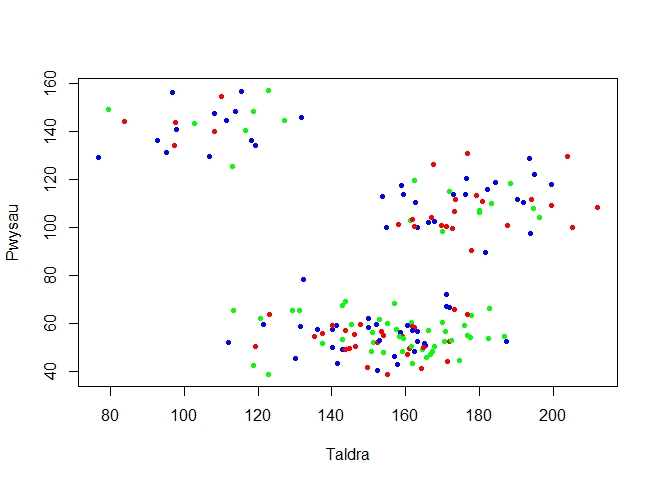
\includegraphics[width=0.5\linewidth]{../img/Cam1.jpeg}
\end{center}
\end{figure}

\item Cyfrifo canolbwynt (hynny yw cymedr) pob clwstwr.

\begin{figure}[H]
\begin{center}
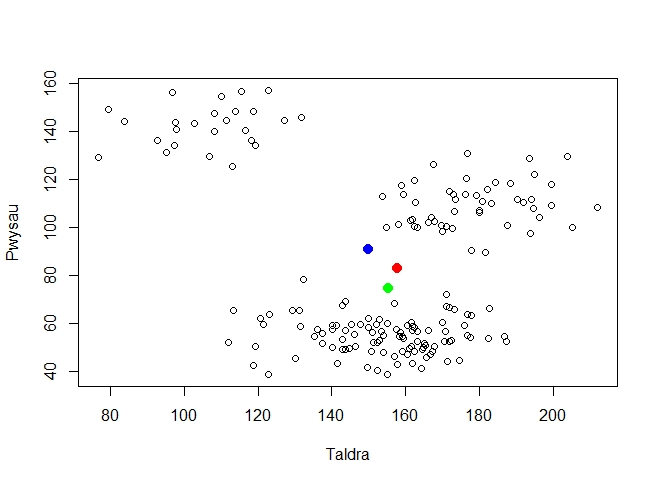
\includegraphics[width=0.5\linewidth]{../img/ClystyrauCychwynol.jpeg}
\end{center}
\end{figure}

\item Ail-aseinio pob elfen unwaith eto i'r clwstwr gyda chymedr agosaf.

\begin{figure}[H]
\begin{center}
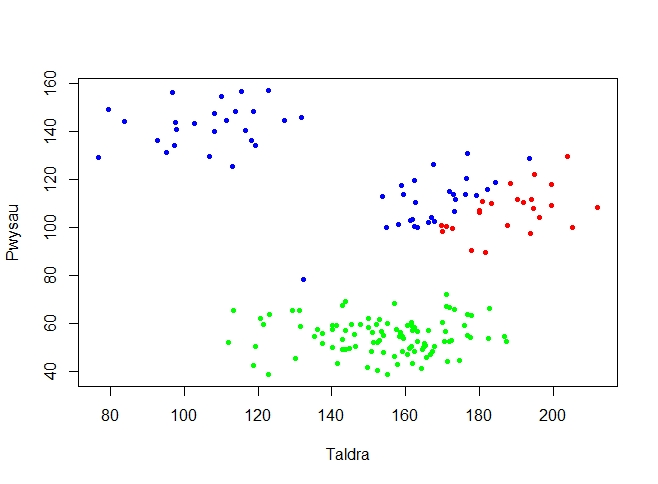
\includegraphics[width=0.5\linewidth]{../img/Cam3.jpeg}
\end{center}
\end{figure}

\item Ailadrodd camau dau a tri tan fod y canolbwyntiau ddim yn symud rhagor.

\begin{figure}[H]
\begin{center}
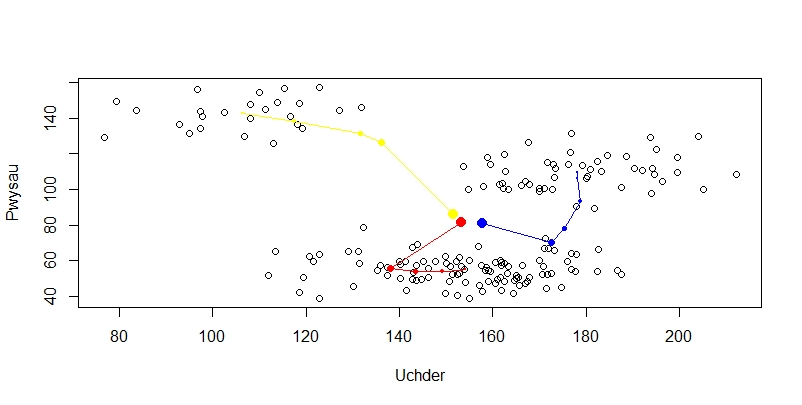
\includegraphics[width=0.5\linewidth]{../img/Convergence4.jpeg}
\end{center}
\end{figure}

\end{enumerate}  

\subsection{Darn Mathemategol} % Angen teitl gwell

Diffiniwn bob clwstwr rydym yn ceisio darganfod fel $C_i$ lle bydd $i \in \{ 1, 2, \dots, k\}$, mae gennym hefyd $n$ pwyntiau data $x_1, x_2, \dots, x_n$. Gadewch i $c_i$ bod yn bwynt sy'n ganolbwynt y clwstwr $C_i$. Ar gyfer y cam cyntaf angen aseinio pob $x_j$ i ryw glwstwr $C_i$ ar hap. Yna gan ein bod yn datgelu ein bod yn delio gyda phl\^{a}n Ewclidaidd, mi fyddem yn darganfod cymedr pob clwstwr gan y fformiwla ganlynol:

\begin{equation}
C_i = \frac{1}{|S_i|}\sum_{x_j \in S_i} {x_j}
\end{equation}

% dyw'r hafaliad hyn ddim yn gwneud synwyr. Ble mae'r $c_i$ y canolbwynt sydd angen. A sut ydych yn symio bwyntiau? Angen mwy o esboniad.

lle diffiniwn $S_i$ fel y set o bwyntiau data sydd wedi'i aseinio i glwstwr $C_i$.

Nawr mae gan bob clwstwr cymedr newydd, fedrwn aseinio pob pwynt data i'r canolbwynt agosaf. Caiff hyn ei gwneud gan fynd drwy bob pwynt data a chyfrifo'r pellter Ewclidaidd i bob canolbwynt. Yna fydd y pwynt priodol yn cael ei labelu gyda'r clwstwr sydd a'r pellter lleiaf o'i chanolbwynt i'r pwynt data. Hynny yw

\begin{equation}
\arg \min_{c_i} dist(c_i, x_j)^2
\end{equation}

Unwaith mae'r proses wedi'i chychwyn, angen ailadrodd y darn o ddarganfod y creiddiau newydd ac yna ail labelu'r pwyntiau data.

% Mae hwn yn swnio fel ond unwaith chi'n ailadrodd y proses. Pryd mae'n gorffen?

\subsection{Sut i ddarganfod y $k$ orau?}

Mae yna wahanol ffurf i ddarganfod $k$, edrychwn ar ddau wahanol ffordd o wneud hyn. 

\subsubsection{Dull Penelin}

Mae'r dull penelin yn cymharu'r cyfanswm o swm sgwariau o fewn y clystyrau. Unwaith gennym y cyfanswm o swm sgwariau o fewn clystyrau i bob $k$ rydym eisiau cymharu, fyddem yn creu plot o bob $k$ yn erbyn y cyfanswm o swm sgwariau o fewn y clystyrau ar gyfer y $k$ hynny. Unwaith mae gennym y graff, allwn ei ddadansoddi. 

% Angen esbonio beth yw swm sgwariau. Oes hafaliad ar ei cyfer?

\begin{figure}[H]
\begin{center}
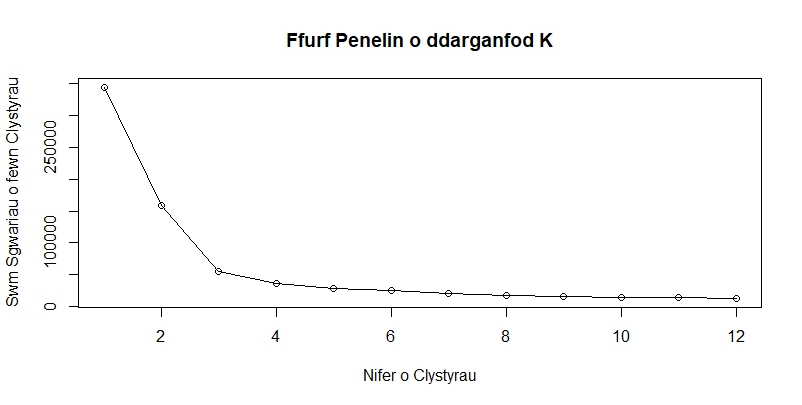
\includegraphics[width=0.5\linewidth]{../img/Dull_Penelin.jpeg}
\end{center}
\caption{Enghraifft o blot o $k$ yn erbyn y cyfanswm swm o sgwariau}
\label{fig:dullpenelin}
\end{figure}

Yn y graff yn Narlun~\ref{fig:dullpenelin}, gwelwn fod swm sgwariau yn fawr yn cychwyn gyda $k$=1 sydd yn gwneud synnwyr. % Pam?
O'r pwynt yma wedyn fydd yna newid mawr yn y swm sgwariau. Unwaith mae'r newid mawr hwn yn dod i ben fydd gennym ongl yn cael ei greu lle bydd newid $k$ dim ond yn creu newid bach. Y pwynt yma fydd yr optimwm ar gyfer nifer $k$ o glystyrau. Fel gwelwn yn glir yn ein henghraifft ni, mae'n glir fod $K$=3 yw dewis orau ar $K$.

\subsubsection{Dendrogram}

Mae dendrogram yn ffordd wahanol iawn i canfod y nifer orau $k$ o glystyrau. Mae'n defnyddio darn o glystyru hierarchaidd i greu diagram canghennog. Mae'r echelin llorweddol yn dangos pob gwrthrych yn ein set o ddata. Mae'r echelin fertigol yn dangos mesur o annhebygrwydd. Mae Darlun~\ref{fig:dendogram} yn dangos dendogram ar gyfer yr un data.

\begin{figure}[H]
\begin{center}
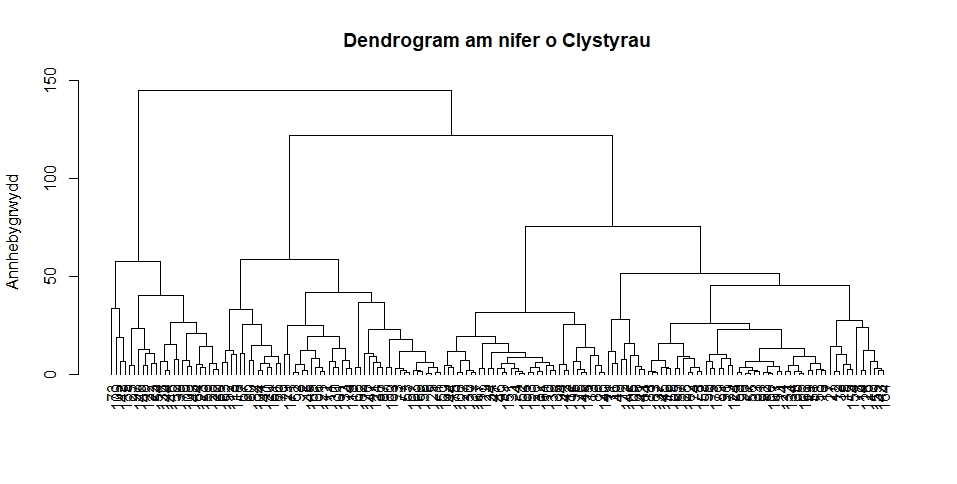
\includegraphics[width=0.5\linewidth]{../img/Dendrogram.jpeg}
\end{center}
\caption{Enghraifft o dendogram}
\label{fig:dendogram}
\end{figure}

I ddadansoddi'r dendrogram mi fyddwn edrych yn bennaf ar yr echelin fertigol. Edrychwn allan am yr annhebygrwydd fwyaf rhwng cyflwyniad o gangen arall yn y goeden. Welwn ni hyn yn ein henghraifft ni ar ôl i'r drydydd clwstwr cael ei gyflwyno yn dendrogram. Mae hyn yn datganu'r un peth a'r dull penelin.

\section{Tiwtorial yn R}
Mi fyddwn yn edrych ar ddata o uchder a phwysau 175 wahanol berson. Mi allwch chi lawrlwytho y data yma o fan hyn. % Cofia ychwanegu'r link

Yno fydd angen lawrlwytho a gosod y pecynnau \mintinline{R}{graphics}, \mintinline{R}{stats} ag \mintinline{R}{datasets} ar eich fersiwn chi o RStudio. Ffordd hawdd i wirio hyn fydd i ddefnyddio'r c\^{o}d canlynol: % Allwn ni neud hwn yn platfform agnostig - h.y. paid sôn am RStudtio, just y cod R. Yna gall unrhywun dilyn rhain lle bynnag mae'n nhw'n rhedeg eu R.

\begin{minted}[bgcolor=green!7]{r}
install.packages("graphics")
install.packages("stats")
install.packages("datasets")
library(graphics)
library(stats)
library(datasets)
\end{minted}

Mae'r darn gyntaf o'r c\^{o}d uchod yn gosod/diweddaru'r pecynnau angenrheidiol. Mae'r ail ddarn yn llwytho'r pecynnau i ein fersiwn ni o RStudio.

Nawr mi wnawn lwytho'r data.

\begin{minted}[bgcolor=green!7]{r}
heightvsweight <- read.csv("C:/Users/User/Desktop/Dysgu_Peirianyddol/heightvsweight.csv")
View(heightvsweight)
\end{minted}

% Gawn ni cael variable names Cymraeg? uchderpwysau?
Mae'r string sydd mewnbwn y ffwythiant \mintinline{R}{read.csv} yn cyfeirio at y lleoliad ar ein cyfrifiadur lle gallwn ganfod y ffeil csv priodol. Rhaid gwneud yn si\^{w}r eich bod yn defnyddio'r lleoliad cywir i'r lleoliad o'ch ffeil chi.
Ar \^{o}l rhedeg y c\^{o}d ddylai eich data edrych yn debyg i'r canlynol: % Cael gwared a'r RStudio reference

\begin{figure}[H]
\begin{center}
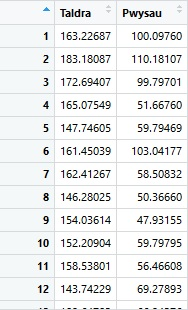
\includegraphics[width=0.35\linewidth]{../img/Data_yn_R.jpg}
\end{center}
\label{fig:DataR}
\end{figure}

Gan fod y data hefo enwau ar gyfer y colofnau, gallwn atodi'r data i lwybr chwilio R. Bydd hyn yn gadael i ni gyfeirio at enwau colofnau'r data yn ein c\^{o}d fydd yn gwneud yn lawer mwy symlach i ddeall.

\begin{minted}[bgcolor=green!7]{r}
attach(heightvsweight)
\end{minted}

I wneud fwy o synnwyr o'r data, mi wnawn blotio'r data.

\begin{minted}[bgcolor=green!7]{r}
plot(Uchder, Pwysau, pch = 21)
\end{minted}

Sy'n rhoi:

\begin{figure}[H]
\begin{center}
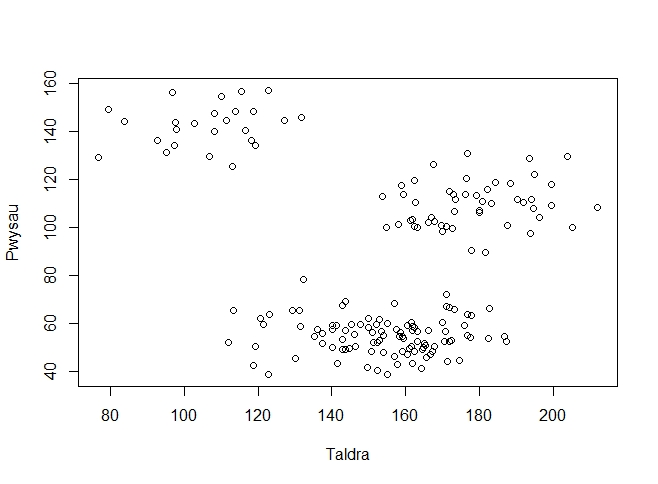
\includegraphics[width=0.5\linewidth]{../img/ScatterplotR.jpeg}
\end{center}
\label{fig:ScatterplotR}
\end{figure}

Gwelwn fod yna 3 clwstwr clir. 

R\^{w}an rydym yn gallu tybio fod y data yn gallu cael i rannu i dri chlwstwr gwahanol, mi wnawn ddefnyddio'r algorithm dysgu peirianyddol i'w ddehongli. Rhedwn y canlynol i redeg clystyru $k$-cymedr yn R. Rydym yn defnyddio'r ymresymiad \mintinline{R}{nstart} i ddewis faint o setiau ar hap o greiddiau wnawn gymered.
% Dydw i ddim yn deall nstart sori. Angen gwell esboniad.

\begin{minted}[bgcolor=green!7]{r}
kcymedr <- kmeans(heightvsweight,3, nstart = 50)
\end{minted}

Allwn nawr adio colofn newydd i'r data sef y clystyrau newydd mae'r algorithm wedi'i darganfod.

\begin{minted}[bgcolor=green!7]{r}
heightvsweight$Clwstwr3 <- kcymedr$cluster
\end{minted}

Gallwn weld y newid hwn gan ddefnyddio'r un c\^{o}d a ddefnyddion yn gynharach.

\begin{minted}[bgcolor=green!7]{r}
View(heightvsweight)
\end{minted}

\begin{figure}[H]
\begin{center}
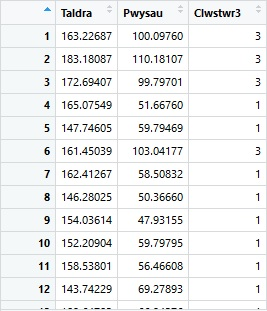
\includegraphics[width=0.5\linewidth]{../img/Data3_yn_R.jpg}
\end{center}
\end{figure}

Mae'n bosib fydd yr algorithm wedi labeli'r clystyrau gwahanol gyda rhifau gwahanol i'r hyn a welwch fan hyn, ddylai'r clystyrau ei hun fod yn hafal. Mae hyn oherwydd y setiau ar hap cychwynnol mae'r algorithm yn ei gymered i gychwyn.

Rhedwn y c\^{o}d canlynol liwio'r clystyrau newydd ar graff.

\begin{minted}[bgcolor=green!7]{r}
plot(Uchder, Pwysau, pch = 21, bg=c("red","green","blue")[unclass(kcymedr$cluster)])
\end{minted}

Sy'n rhoi:

\begin{figure}[H]
\begin{center}
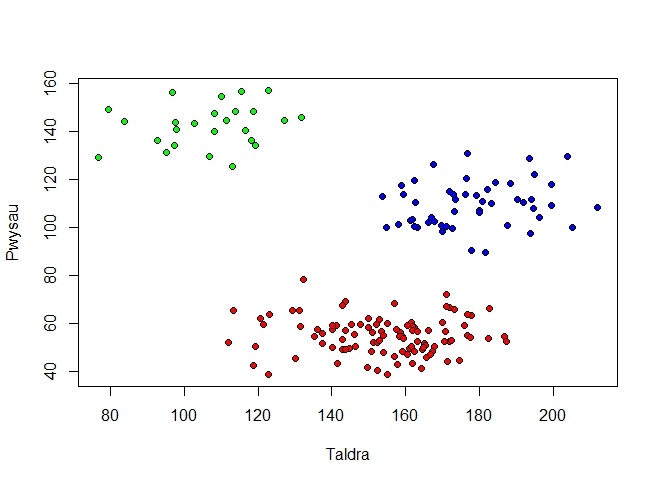
\includegraphics[width=0.5\linewidth]{../img/3clwstwrR.jpeg}
\end{center}
\end{figure}

I gymharu, nawr mi nawn rhedeg yr algorithm ar gyfer 6 clwstwr i weld y clystyrau pan fydd $k=6$. 

\begin{minted}[bgcolor=green!7]{r}
kcymedr <- kmeans(heightvsweight,6, nstart = 50)
heightvsweight$Clwstwr6 <- kcymedr$cluster
View(heightvsweight)
\end{minted}

\begin{figure}[H]
\begin{center}
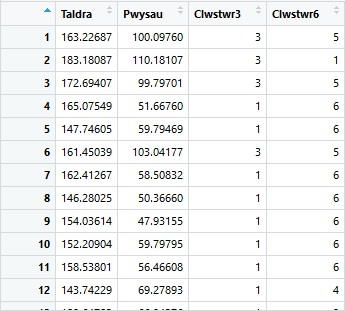
\includegraphics[width=0.5\linewidth]{../img/Data6_yn_R.jpg}
\end{center}
\end{figure}

Gwelwn fod y labeli newydd wedi cael ei ychwanegu i'n tabl. Yna gan blotio graff arall, fedrem weld y 6 clwstwr yn gliriach.

\begin{minted}[bgcolor=green!7]{r}
lliwiau <- c("red","green","blue", "yellow", "black", "white")
plot(Uchder, Pwysau, pch = 21, bg=lliwiau[unclass(kcymedr$cluster)])
\end{minted}

Sy'n rhoi:

\begin{figure}[H]
\begin{center}
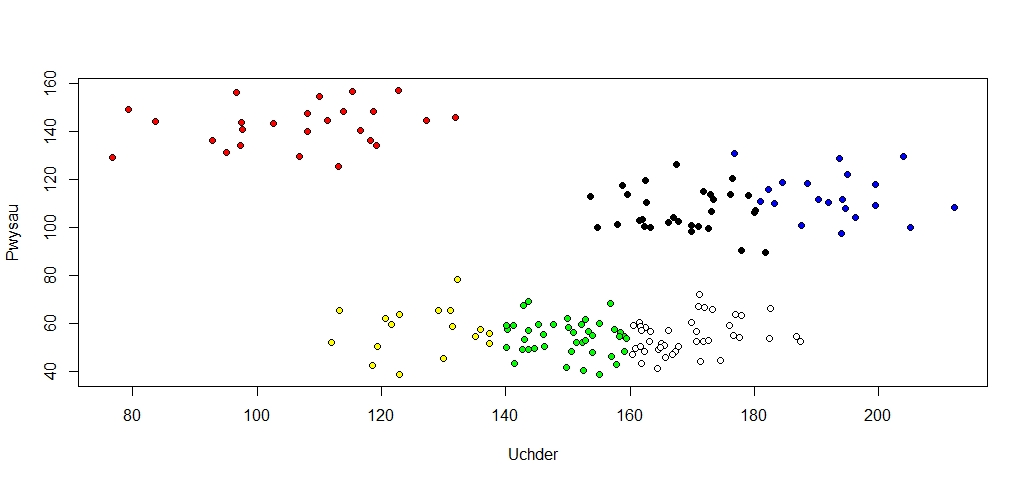
\includegraphics[width=0.5\linewidth]{../img/6clwstwrR.jpeg}
\end{center}
\end{figure}


%Mae'r data iris ar gael iddym drwy'r pecyn "datasets". Yn yr enghraifft top mi wnaethom defnyddio k fel 3, felly hyna be wnawn neud eto.
%Dyma'r c\^{o}d ar gyfer rhedeg clystyru k-cymedr:
%\begin{minted}[bgcolor=green!7]{r}
%clysteru_tri <- kmeans(iris[,1:4],3, nstart = 20)
%clysteru_tri 
%\end{minted}
%Mae'r llinell gyntaf o c\^{o}d yn rhedeg clystyru k-cymedr ar y set data iris gyda k=3. Mae'r darn nstart yn cynrychioli faint o dosraniadau i drio yn cychwyn yn erbyn'r ffwythiant amcan, er mwyn dewis y cychwyn orau. Mae'r ail linell yn allbwn yr wybodaeth canlynol:
%\begin{minted}[bgcolor=green!7]{r}
%>>>K-means clustering with 3 clusters of sizes 50, 62, 38
%>>>
%>>>Cluster means:
%>>>  Sepal.Length Sepal.Width Petal.Length
%>>>1     5.006000    3.428000     1.462000
%>>>2     5.901613    2.748387     4.393548
%>>>3     6.850000    3.073684     5.742105
%>>>  Petal.Width
%>>>1    0.246000
%>>>2    1.433871
%>>>3    2.071053
%>>>
%>>>Clustering vector:
%>>>  [1] 1 1 1 1 1 1 1 1 1 1 1 1 1 1 1 1 1 1 1 1 1 1
%>>> [23] 1 1 1 1 1 1 1 1 1 1 1 1 1 1 1 1 1 1 1 1 1 1
%>>> [45] 1 1 1 1 1 1 2 2 3 2 2 2 2 2 2 2 2 2 2 2 2 2
%>>> [67] 2 2 2 2 2 2 2 2 2 2 2 3 2 2 2 2 2 2 2 2 2 2
%>>> [89] 2 2 2 2 2 2 2 2 2 2 2 2 3 2 3 3 3 3 2 3 3 3
%>>>[111] 3 3 3 2 2 3 3 3 3 2 3 2 3 2 3 3 2 2 3 3 3 3
%>>>[133] 3 2 3 3 3 3 2 3 3 3 2 3 3 3 2 3 3 2
%>>>
%>>>Within cluster sum of squares by cluster:
%>>>[1] 15.15100 39.82097 23.87947
%>>> (between_SS / total_SS =  88.4 %)
%\end{minted}
%Mae'r c\^{o}d uchod rhoi pob wybodaeth a fysa chi eisiau wybod fel allbwn o'r proses.
%I weld y clysterau allwn plotio graff ar gyfer phob cyfuniad o newidynnau. Mae hyn yn alluogi ni i weld yr gwaith dpsbarthu mae'r algorithm wedi'i neud.
%\begin{minted}[bgcolor=green!7]{r}
%plot(iris[,1:4], pch = 24, bg=c("red","green3","blue")[unclass(clysteru_tri$cluster)])
%\end{minted}
%Yn y ffwythiant "plot" uchod, mae'r darn gynta ohono yn cyfeirio tuag at pa data fydd yn cael ei clysteru. Mae'r ail darn yn penodi be fydd pob pwynt data yn cael ei cynrychioli fel pan %mae'r darn dwythaf yn penodi lliw i pob clwstwr.

%Mi wnawn edrych y nawr ar yr set data iris sy'n boblogaidd iawn yn y maes ystadegaeth a gwyddor data. Mae'r data yn cynnwys mesuriadau uchder ag lled petal a setal 150 planhigyn iris. Yn isod gweler lun o allbwn clystyru k-cymedr yn erbyn y clystyrau gwreiddiol o'r data. Gwelwyd fod yr algorithm yn neud yn wych!


\section{Tiwtorial yn python}
Yn y tiwtorial hwn mi wnawn edrych ar yr un data a welom yn y tiwtorial diwethaf.
I gychwyn bydd rhaid llwytho'r pecynnau \mintinline{python}{pandas}, \mintinline{python}{matplotlib.pyplot} ag \mintinline{python}{sklearn.cluster} drwy redeg y c\^{o}d canlynol:

\begin{minted}[bgcolor=cyan!7]{python}
import pandas as pd
import matplotlib.pyplot as plt
import sklearn.cluster
\end{minted}

Y r\^{w}an mi wnawn lwytho'r data i mewn i'n gwaith gan redeg y c\^{o}d:

\begin{minted}[bgcolor=cyan!7]{python}
data = pd.read_csv('heightvsweight.csv')
\end{minted}

Mae'r string sydd mewnbwn y ffwythiant \mintinline{R}{pd.read_csv} yn cyfeirio at y lleoliad ar ein cyfrifiadur lle gallwn ganfod y ffeil csv priodol. Rhaid gwneud yn si\^{w}r eich bod yn defnyddio'r lleoliad cywir i'r lleoliad o'ch ffeil chi.
Unwaith fydd wedi cael ei llwytho, allwn ni gweld yn fras y data gennym ni. 

\begin{minted}[bgcolor=cyan!7]{python}
data.head()
\end{minted}

\begin{figure}[H]
\begin{center}
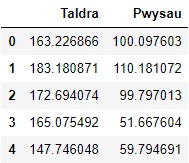
\includegraphics[width=0.35\linewidth]{../img/tabl1.jpg}
\end{center}
\label{fig:Data1}
\end{figure}

I weld y data mewn ffordd fwy gweledol, wnawn blotio graff gwasgariad o'r data

\begin{minted}[bgcolor=cyan!7]{python}
plt.scatter(data['Uchder'], data['Pwysau']);
plt.xlabel('Uchder')
plt.ylabel('Pwysau')
plt.show()
\end{minted}

\begin{figure}[H]
\begin{center}
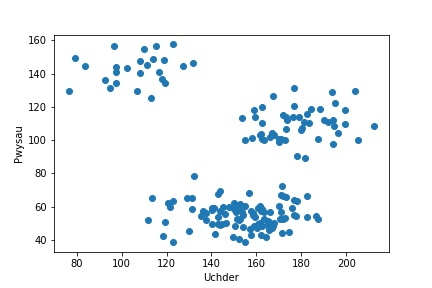
\includegraphics[width=0.7\linewidth]{../img/Scatterpython.jpeg}
\end{center}
\caption{Enghraifft o ddata da i cael ei clystyru.}
\label{fig:Scatterpython}
\end{figure}

Fel gwelwn, mae'r data yn edrych fel ei fod mewn tri chlwstwr. Felly wnawn ddefnyddio'r ffurf algorithm dysgu peirianyddol i'w labelu.

\begin{minted}[bgcolor=cyan!7]{python}
kmeans = sklearn.cluster.KMeans(n_clusters=3).fit(data)
data['Cluster (k=3)'] = kmeans.predict(data)
\end{minted}

Gallwn weld y newid hwn gan ddefnyddio'r un c\^{o}d a ddefnyddion yn gynharach.

\begin{minted}[bgcolor=cyan!7]{python}
data.head()
\end{minted}

\begin{figure}[H]
\begin{center}
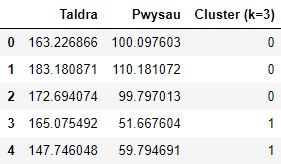
\includegraphics[width=0.35\linewidth]{../img/tabl2.jpg}
\end{center}
\label{fig:Data2}
\end{figure}

Fel y gwelwyd, mae'r data wedi'i rhoi i mewn i dri chlwstwr ac wedi'i labelu gyda rhif y clwstwr. Gan fod pob pwynt yn y data nawr gyda label, allwn ni creu'r plot eto ond gyda bob clwstwr yn lliw gwahanol.

\begin{minted}[bgcolor=cyan!7]{python}
plt.scatter(data['Uchder'], data['Pwysau'], c=data['Cluster (k=3)']);
plt.xlabel('Uchder')
plt.ylabel('Pwysau')
plt.show()
\end{minted}

Sy'n rhoi:

\begin{figure}[H]
\begin{center}
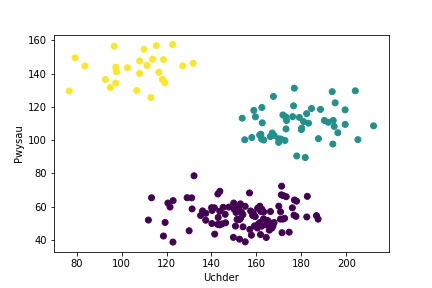
\includegraphics[width=0.7\linewidth]{../img/3clystwrpython.jpeg}
\caption{Sut ddylsa eich graff edrych gyda 3 clystwr.}
\label{fig:3clystwrpython}
\end{center}
\end{figure}

Fel y gwelwn, gweithiodd yr algorithm yn wych. Wnawn nawr trio clystyru $k$-cymedr gyda $k$ yn hafal i 6.

\begin{minted}[bgcolor=cyan!7]{python}
kmeans = sklearn.cluster.KMeans(n_clusters=6).fit(data)
data['Cluster (k=6)'] = kmeans.predict(data)
\end{minted}

Sy'n rhoi:

\begin{minted}[bgcolor=cyan!7]{python}
data.head()
\end{minted}

\begin{figure}[H]
\begin{center}
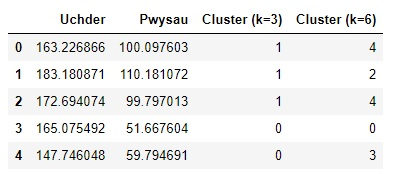
\includegraphics[width=0.35\linewidth]{../img/tabl3.jpg}
\end{center}
\label{fig:Data3}
\end{figure}

Gallwn hefyd gweld canlyniad rhoi'r data i mewn i 6 clwstwr gwahanol: 

\begin{minted}[bgcolor=cyan!7]{python}
plt.scatter(data['Uchder'], data['Pwysau'], c=data['Cluster (k=6)']);
plt.xlabel('Uchder')
plt.ylabel('Pwysau')
plt.show()
\end{minted}

Sy'n rhoi:

\begin{figure}[H]
\begin{center}
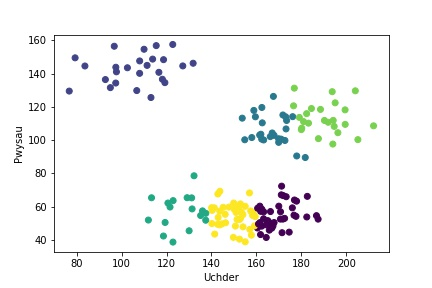
\includegraphics[width=0.7\linewidth]{../img/6clystwrpython.jpeg}
\caption{Sut ddylsa eich graff edrych gyda 6 clystwr.}
\label{fig:6clystwrpython}
\end{center}
\end{figure}

Dyma sut dylaf eich data edrych fel ar \^{o}l a phrosesu drwy glystyru 6-cymedr. 

